%% LyX 2.0.5.1 created this file.  For more info, see http://www.lyx.org/.
%% Do not edit unless you really know what you are doing.
\documentclass[usenatbib]{article}
\usepackage[latin9]{inputenc}
\usepackage[a4paper]{geometry}
\geometry{verbose}
\usepackage{color}
\usepackage{float}
\usepackage{graphicx}

\makeatletter

%%%%%%%%%%%%%%%%%%%%%%%%%%%%%% LyX specific LaTeX commands.
%% A simple dot to overcome graphicx limitations
\newcommand{\lyxdot}{.}


%%%%%%%%%%%%%%%%%%%%%%%%%%%%%% Textclass specific LaTeX commands.
\usepackage{jcappub}

%%%%%%%%%%%%%%%%%%%%%%%%%%%%%% User specified LaTeX commands.






%%%%%%%%%%%%%%%%%%%%%%%%%%%%%% LyX specific LaTeX commands.
%% A simple dot to overcome graphicx limitations
%Make my life significantly easier
\global\long\def\bd{{\bm{\delta}}}

\usepackage{astrobib_mnras2e}

\bibliographystyle{JHEP}

\makeatother

\begin{document}

\title{The Maximum Circular Velocity Dependence of Halo Clustering}

\maketitle

\section{Introduction}

\textcolor{black}{The halo model} has been remarkably successful in
describing observations of galaxy clustering. In particular, the Halo
Occupation Distribution (HOD) and the Conditional Luminosity Function
(CLF) have been widely used to constrain not only the galaxy-halo
connection {[}XXX{]} but also cosmology {[}XXX{]}. The fundamental
assumption in both formalisms is that galaxy occupation statistics
only depends on halo mass. 

The spatial distribution of dark matter (DM) halos in N-body simulations,
however, exhibits dependence on halo mass as well as on additional
properties such as halo formation time {[}XXX{]}. The dependence of
halo clustering upon other properties besides halo mass known as halo
assembly bias. \textcolor{black}{There have been several studies showing
the correlation between halo formation time and environment, and therefore
any other properties which depends on formation time or environment
(such as concentration, spin, and velocity anisotropy) affect to the
assembly bias. This assembly bias violates the standard HOD/CLF assumption
and also questions how these model can predict the clustering statistics
of galaxies correctly.}

As a response to halo assembly bias, recent trend in the way to populate
galaxies has been to use the Abundance Matching technique based on
the maximum circular velocities of halos. The motivation behind use
of the maximum circular velocity is that it depends only on the central
part of the halo potential (i.e., potentially more closely related
to galaxy formation) and sets early in the growth of the halo {[}XXX:
Frank's paper{]} (i.e., more robust to disruption in mergers).

In this paper, we explore the dependence of galaxy clustering on the
central velocity dispersion both on small and large scales. We show
that some of the features on small scales in a detailed halo model
come from the effects of back-splash halos, which is one of the categories
of halos classified based on the halo merger tree.


\section{The Simulation}

We use cosmological N-body simulations called the Bolshoi simulation
and the MultiDark simulation, described in XXX and XXX respectively,
to investigate the maximum circular velocity dependence of halo clustering.
The Bolshoi simulation uses $2048^{3}$ particles with a volume of
$(250$$h^{-1}{\rm Mpc})^{3}$, while the MultiDark simulation uses
the same number of particles as the Bolshoi simulation but with a
volume of ($1h^{-1}{\rm Gpc})^{3}$. Both simulations assumes a flat
$\Lambda{\rm CDM}$ model with density parameters $\Omega_{m}=0.27$,
$\Omega_{\Lambda}=0.73$, $\Omega_{b}=0.0469$, and $\sigma_{8}=0.82$,
$n=0.95$, $h=0.70$. The details of the simulations are described
in XXX. We use both simulations to get a large dynamic mass range.

For halo identification, we use the ROCKSTAR halo finder (XXX) where
the halo masses and maximum circular velocities are computed from
bound particles. For the sake of the internal structure of halos to
be resolved well enough, we make a conservative cut in mass and maximum
circular velocity. We use halos whose mass is greater than $10^{12}h^{-1}{\rm M_{\odot}}$
(corresponding to $>100$ particles per halo) and whose maximum circular
velocity is greater than $200{\rm km/s}$ for the MultiDark simulation,
and halos whose mass is greater than $10^{11}h^{-1}{\rm M_{\odot}}$
(corresponding to $>740$ particles per halo) and whose maximum circular
velocity is greater than $95{\rm km/s}$ for the Bolshoi simulation.
Those values correspond to the peak in the number of halos by binning
them as a function of mass and maximum circular velocity. 

From the merger tree, we can classify halos into three different categories:
host halo, subhalos, and ejected halos. Host halos are the halos which
have never been within the virial radius of more massive halos. Subhalos
are the halos which are within the virial radius of more massive halos
at $z=0$. Ejected halos, sometimes called ``backsplash'' halos,
are the distinct halos at $z=0$ whose main progenitors passed through
the virial radius of a more massive halos at least once in the past.
In later sections, when we say halos without any specifications, we
include both host halos and ejected halos. 


\section{The Maximum Circular Velocity Dependence of Halo Clustering}

In this section, we investigate the maximum circular velocity dependence
of halo clustering on both large and small scales. We first start
with an analytic expression of the maximum circular velocity computed
from the halo mass and its concentration. Then, we explain how we
select halos for each sample to remove the halo mass dependence using
the analytic expression of the maximum circular velocity. Finally,
we show how halo biases differ for those samples both on large scales
and small scales.


\subsection{The Maximum Circular Velocity}

In order to compute the maximum circular velocity for halos, we assume
that dark matter halos are defined as a spherical halo with a virial
radius. Those halos have average density equal to $\Delta_{{\rm h}}\rho_{{\rm crit}}$
where $\Delta_{{\rm h}}=360$ for the MultiDark and Bolshoi simulations.
We also assume that those spherical halos have an NFW density profile
(XXX). Then, the maximum circular velocity $\overline{V}_{{\rm max}}$
as a function of the halo mass $M_{{\rm vir}}$ and its concentration
$c$ is given by:

\begin{equation}
\overline{V}_{{\rm max}}=0.465M_{{\rm vir}}^{1/3}\sqrt{G(\frac{4}{3}\pi\Delta_{{\rm h}}\rho_{{\rm crit}}\Omega_{m})^{1/3}\frac{c}{{\rm ln(1+c)-c/(1+c)}}}.\label{eq:vmax-mvir}
\end{equation}
The median concentration-mass relation at $z=0$ obtained from the
Bolshoi simulation in Ref. XXX(Klypin et al. 2011) is: 
\begin{equation}
{\rm log}_{10}c=-0.097{\rm log_{10}M_{vir}}+2.148.\label{eq:concen}
\end{equation}
\textcolor{black}{By using the above median concentration to Eq. \ref{eq:vmax-mvir},
we obtain a one to one mapping between the virial halo mass and its
maximum circular velocity, denoted as $\overline{V}_{{\rm max}}$
hereafter.} Given this mapping, we can translate clustering measurements
as a function of halo mass into predicted clustering measurements
as a function of maximum circular velocity. Our goal below is to determine
whether this conversion describes the measured clustering or if there
is a residual dependence on the maximum circular velocity.


\subsection{Samples}

\begin{figure}
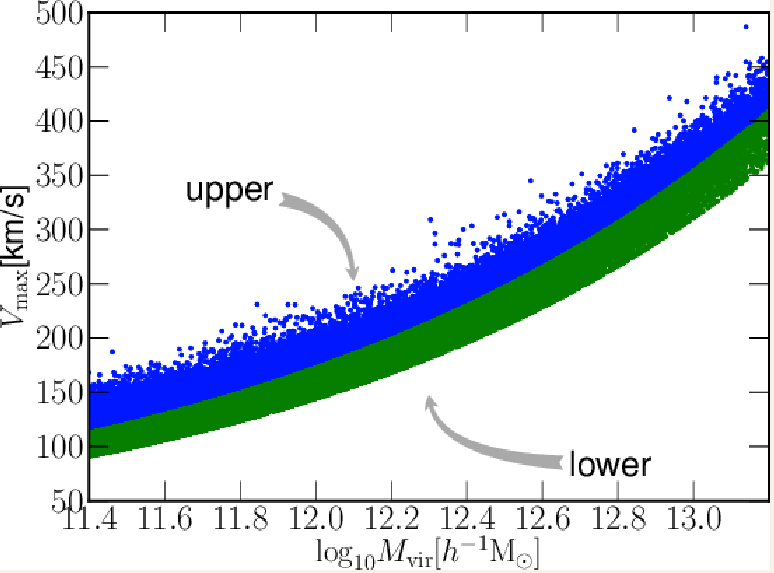
\includegraphics[width=0.5\columnwidth]{/Users/old_ts485/Desktop/biasVmax/plots/plaecholder}\caption{\label{fig:vmax-mvir}Distribution of halo mass and maximum circular
velocity at $z=0.0$ for halos\textcolor{black}{{} from the Bolshoi
simulation.} The blue dots represent halos whose observed maximum
circular velocity, $V_{{\rm max,obs}}$, is greater than $\overline{V}_{{\rm max}}$,
while the green dots are the ones with smaller $V_{{\rm max,obs}}$
than $\overline{V}_{{\rm max}}$. The boundary between blue and green
dots correspond to $\overline{V}_{{\rm max}}$ computed from Eq. \ref{eq:vmax-mvir}.}
\end{figure}


We first split the sample into a sequence of virial mass bins, chosen
such that there are the same numbers of halos in each bin. This process
is reminiscent of an abundance matching procedure (cite XXX). We then
further split each bin into two subsamples with their observed $V_{{\rm max,obs}}$
greater than (denoted by ``upper'') or less than (denoted as ``lower'')
$\overline{V}_{{\rm max}}$. Fig. \ref{fig:vmax-mvir} shows the distribution
of halo mass and maximum circular velocity classified into ``upper''
(blue dots) and ``lower'' (green dots) samples as an example. Note
that the number of halos in ``upper'' and ``lower'' subsamples\textcolor{black}{{}
are }almost equal for any halo mass bins. This selection ensures that
both the upper and lower subsamples have the same mean halo mass.
Therefore, in the absence of an additional $M_{{\rm vir}}$ dependence
on clustering, these samples should have the same clustering properties.
Note that this would not be true if we had simply split the sample
along $V_{{\rm max}}$, since the two resulting subsamples would have
different mean halo masses. 


\subsection{Halo Bias}

In order to measure halo biases, we first compute halo-matter cross
correlation functions for each subsample. We use cross correlation
functions to reduce the shot noise effect on the error. Here, instead
of using full DM particles, we subsample $10^{6}$ particles to compute
the cross correlation functions and matter auto correlation functions.
Then, we define a linear bias: 
\begin{equation}
b_{{\rm lin}}=\sum_{i}(\xi_{hm}(r_{i})/\xi_{mm}(r_{i}))/N_{{\rm bin}},
\end{equation}
where $\xi_{hm}$ and $\xi_{mm}$ are halo-matter and matter-matter
correlation functions and we take the average of the ratio on $r$
from $10h^{-1}{\rm Mpc}$ to $20h^{-1}{\rm Mpc}$, which contains
20 bins in total. 

Fig. \ref{fig:linear-bias} shows linear biases as a function of halo
mass by splitting each sample into ``upper'' and ``lower'' subsamples.
For large halo masses, the ``lower'' subsamples have larger linear
biases than the ``upper'' subsamples. This result is consistent
with the result discusses in Ref. XXX(Dalal et al. 2008). For low
halo masses, the ``upper'' subsamples have larger linear biases
than the ``lower'' subsamples. Those halos which have larger maximum
circular velocities than $\overline{V}_{{\rm max}}$ are the ones
which are supposed to grow into larger mass halos, but somehow the
mass growth is suppressed. This is why those halos in the ``upper''
subsamples cluster more strongly than the ones in the ``lower''
subsamples. As halo mass decreases, the difference in linear bias
between the ``upper'' and ``lower'' subsamples increases up to
$\sim40\%$. On low mass end, there is a drop in the ratio of the
linear biases. We think that the drop is due to mass resolution of
the simulation.

\begin{figure}
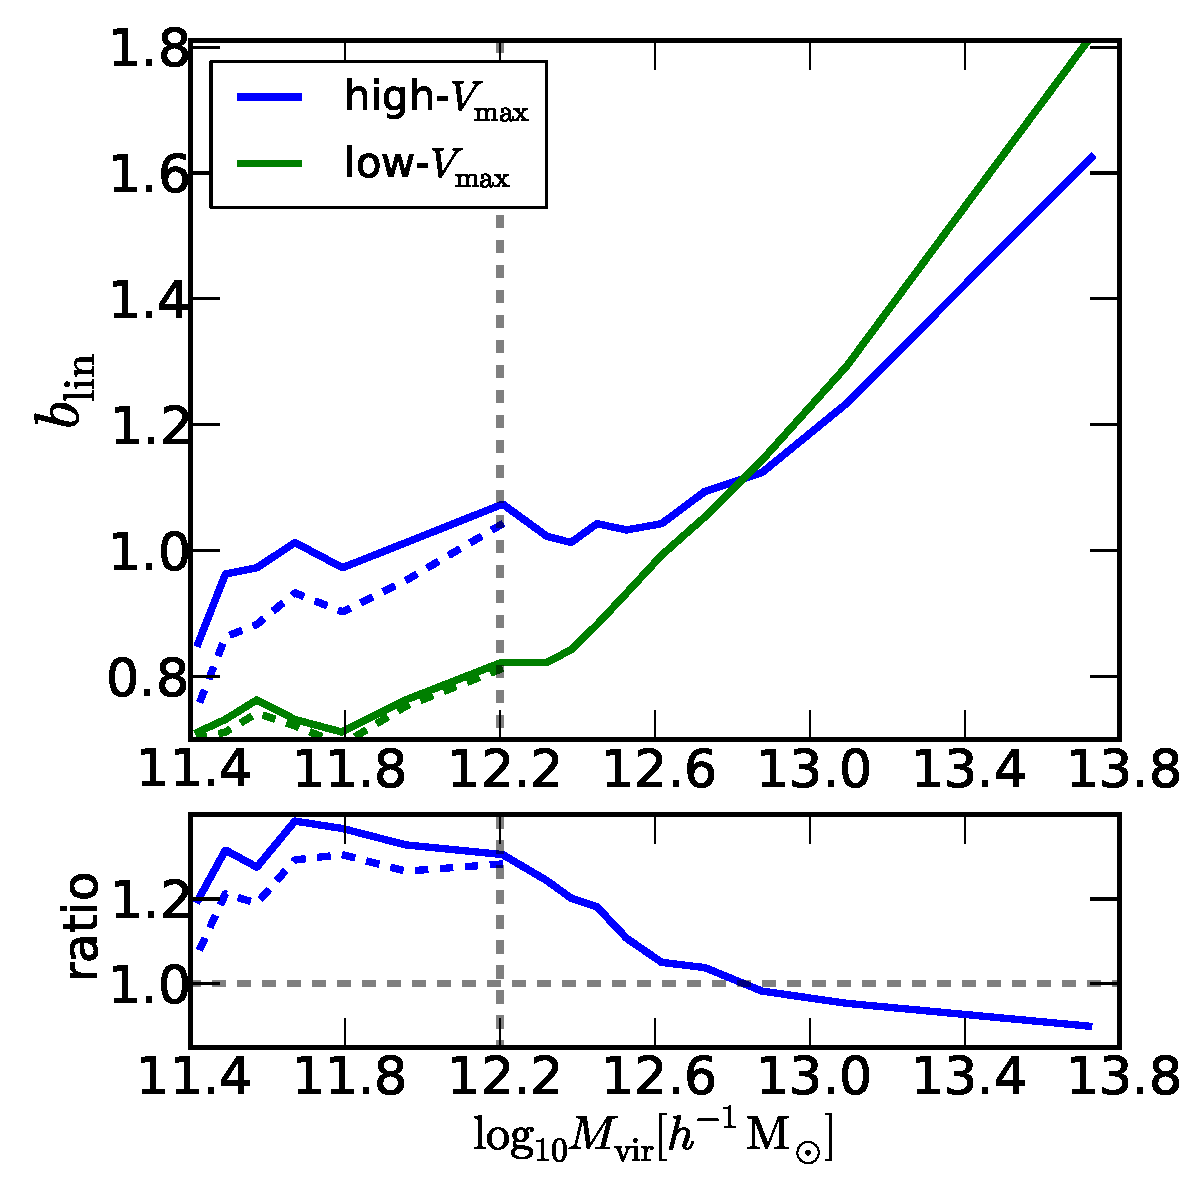
\includegraphics[width=0.5\columnwidth]{/Users/old_ts485/Desktop/biasVmax/plots/linearBias_wang}

\caption{\label{fig:linear-bias}Upper panel: Linear bias at $z=0.0$ as a
function of halo mass from the Bolshoi simulation (circle points)
and the MultiDark simulation (triangle points). The blue circles corresponds
to a linear bias for halos whose maximum circular velocities are greater
than $\overline{V}_{{\rm max}}$ (called ``upper'' samples in the
text), while the green circles correspond to halos whose maximum circular
velocities are smaller than $\overline{V}_{{\rm max}}$ (called ``lower''
samples). Lower panel: Ratio of linear biases between ``upper''
(i.e., $V_{{\rm max}}>\overline{V}_{{\rm max}}$) and ``lower''
(i.e., $V_{{\rm max}}<\overline{V}_{{\rm max}}$) samples from the
Bolshoi simulation and the MultiDark simulation. As halo masses decrease,
the difference on linear bias between ``upper'' and ``lower''
samples becomes larger up to 40\%. .}
\end{figure}


Although halo biases are constant on large scales, halo biases on
small scales are scale-dependent (XXX:reference). We explore whether
the ``upper'' and ``lower'' subsamples have different scale-dependence
in small scale halo biases. In order to explore that, we take the
ratio of the cross correlation functions between the ``upper'' and
``lower'' subsamples and normalize it with their linear biases.
Fig. \ref{fig:small-scale} shows the ratios for several mass bins.
The first three mass bins labeled in the figure, ${\rm log_{10}M[h^{-1}{\rm M_{\odot}}]=11.7,12.0,12.2}$,
are from the Bolshoi simulation, and the last two mass bins, ${\rm log_{10}M[h^{-1}{\rm M_{\odot}}]=12.7,13.1}$,
are from the MultiDark simulation. The ``upper'' and ``lower''
subsamples have very different scale-dependence, especially around
1 to 2$h^{-1}{\rm Mpc}$. Furthermore, the difference on small scales
becomes larger for lower halo mass samples\textcolor{black}{. This
implies that those low mass halos in the ``upper'' subsamples cluster
strongly and likely to live in hot environments near massive halos.}

Up to now, we use both host halos and ejected halos to compute halo
biases. Both types of halos are identified as distinct halos at $z=0$.
Ejected halos, however, are halos which were identified as part of
more massive halos at one or more occasions in the past. Those ejected
halos tend to exist around more massive halos (any reference?), and
only some of them may be gravitationally bound to other more massive
halos. Therefore, the efect on the scale-dependent biases may be caused
by those ejected halos. To test this, we compute halo-matter cross
correlation functions without the ejected halos. Similar to Fig. \ref{fig:linear-bias},
we first compare linear biases as a function of halo mass. We observe
that the ratios of linear biases between the ``upper'' and ``lower''
subsamples are suppressed by $\sim10\%$. Next, we compare cross correlation
functions on small scales, as shown in Fig. \ref{fig:eject}, similar
to what was done in Fig. \ref{fig:small-scale}. Fig. \ref{fig:eject}
only shows the results for low mass halos from\textcolor{black}{{} the
Bolshoi simulation. This is because} we do not find many ejected halos
in the MultiDark simulation due to its mass resolution. \textcolor{black}{Once
the ejected halos have been removed, the deviation of the halo bias
on small scales is greatly reduced. }This implies an intimate connection
between assembly bias and subhalo back-splashing.

We conclude that halos which have different $V_{{\rm max}}$ cluster
differently even when those halos have the same virial mass. In particular,
the scale-dependence of halo biases on small scales is significantly
different, which is mainly caused by the ejected halos. 

\begin{figure}[H]
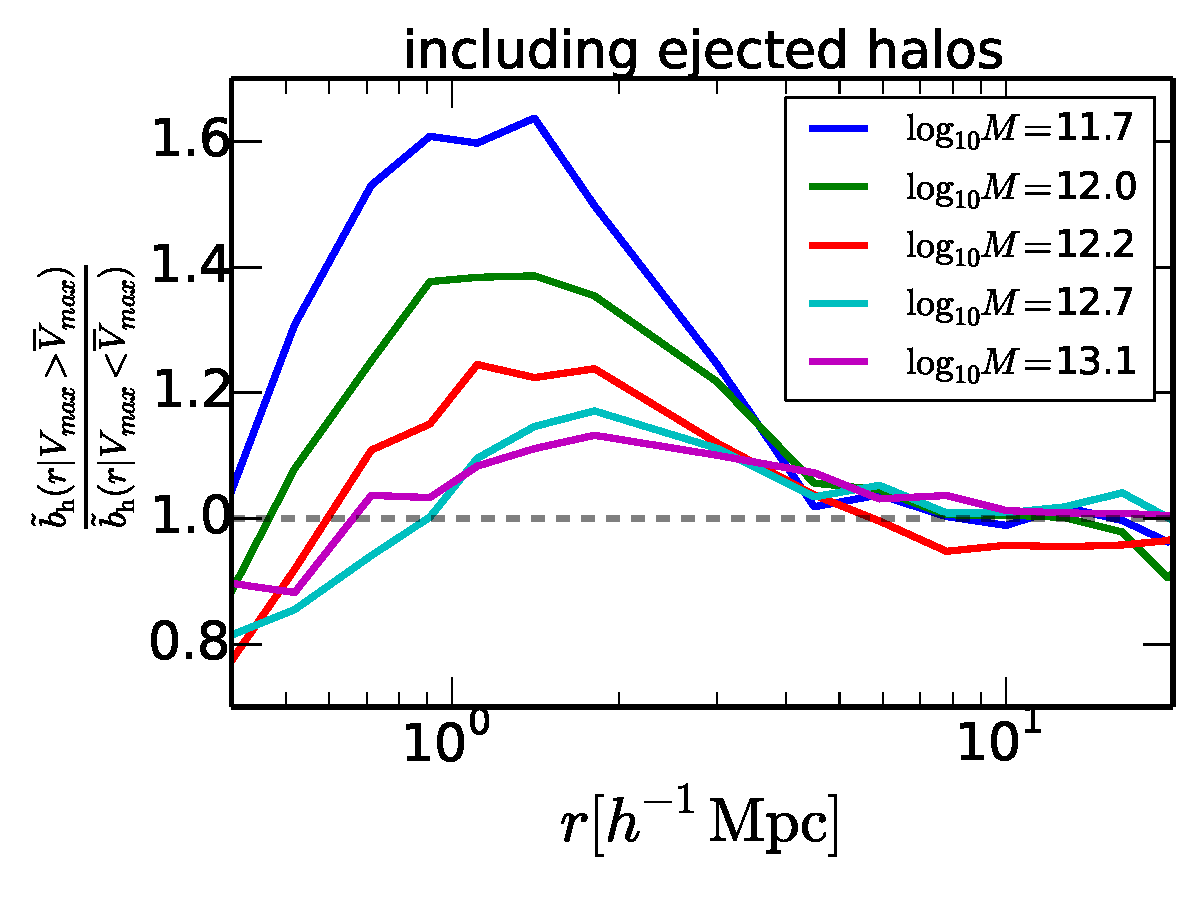
\includegraphics[width=0.8\columnwidth]{/Users/old_ts485/Desktop/biasVmax/plots/Both_smallScale_wang_log}

\caption{\label{fig:small-scale}Ratio of halo-matter cross correlation functions
between ``upper'' and ``lower'' subsamples normalized by their
linear biases. The plots are from the Bolshoi simulation and the MultiDark
simulation at z = 0.0. Each line corresponds to different halo mass
bins labeled in the plots. Those plots show that ``upper'' and ``lower''
subsamples have different scale-dependence on small scales and the
relative scale-dependence between those subsamples increases smoothly
with decreasing halo mass. which lines come from MD...}


\end{figure}


\begin{figure}[H]
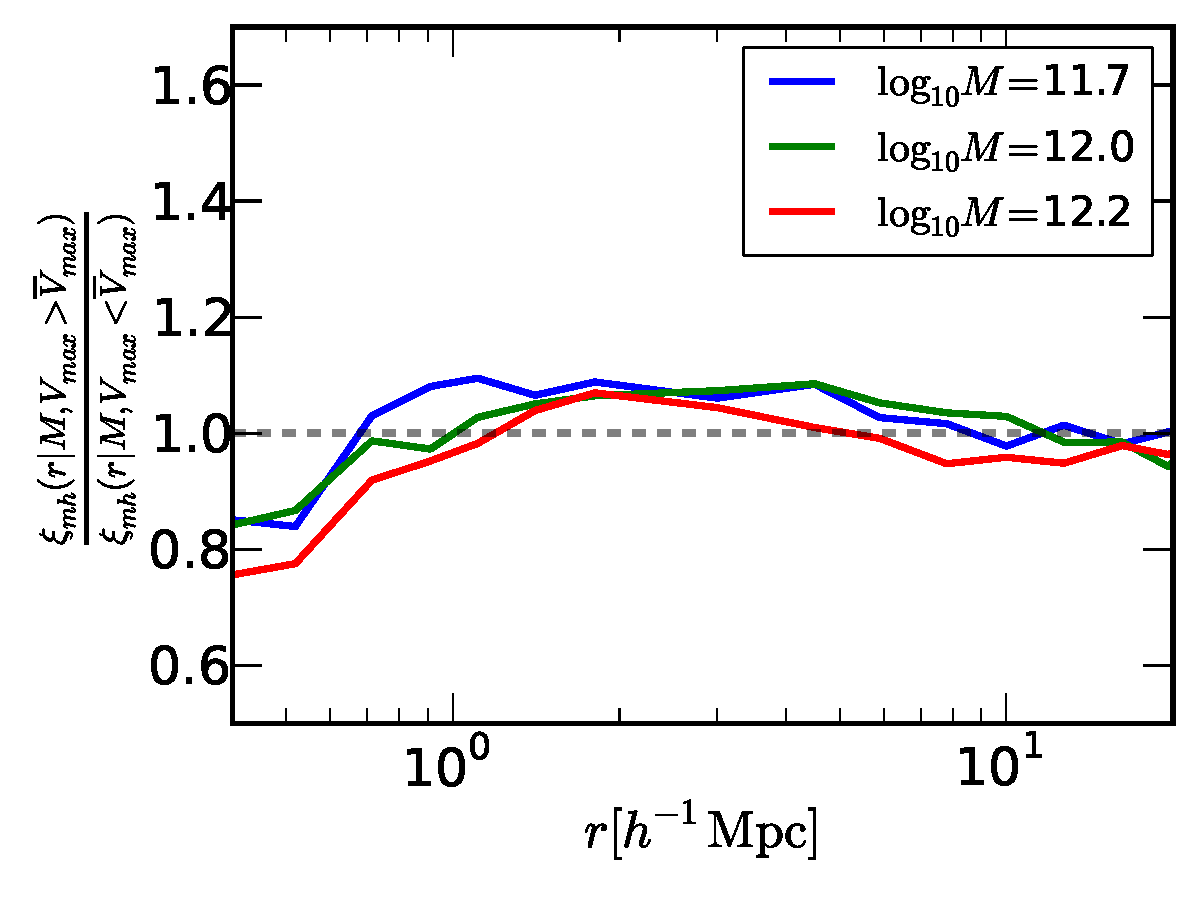
\includegraphics[width=0.5\columnwidth]{/Users/old_ts485/Desktop/biasVmax/plots/Bolshoi_smallScale_wang_log_eje}

\caption{\label{fig:eject}The same figures as Fig. \ref{fig:small-scale}
without ejected halos only from the Bolshoi simulation. As can be
seen by comparing these results to those in Fig. \ref{fig:small-scale},
the $V_{{\rm max}}$-dependence of halo bias on small scales is dramatically
reduced by excluding ejected subhalos. This implies an intimate connection
between assembly bias and subhalo back-splashing.}


\end{figure}


--use jackknife sampling to put error bars


\section{Applications}

In this section, we demonstrate \textcolor{black}{possible observational
relevances of the results in the previous section to complement the
halo theory results. }We start with the abundance matching (citation?)
technique based on halo mass and the maximum circular velocity, and
then compute $\Delta\Sigma({\rm R})$ using those two different abundance
matching techinique.


\subsection{Mvir-based v.s. Vmax-based}

In abundance matching, we link galaxy populations to halo populations
by assuming that big galaxies live in big halos in a hierarchical
manner. The question is what ``big'' halos really means. To rank
order halos, we want to identify what kind of physical properties
characterize halo ``size''. As a first step, we explore how the
abundance matching based on halo mass and maximum circular velocity
influence halo clustering.

Similar to the previous section, we compute halo-matter cross correlation
functions for the abundance matched samples by splitting halos into
a sequence of halo mass bins, $\overline{n}(M_{{\rm vir}})$, and
the maximum circular velocity bins, $\overline{n}(V_{{\rm max}})$,
chosen such that each bin has the same number of halos. We observe
that when we include ejected halos, the linear biases for the $V_{{\rm max}}$-samples
are larger than the ones for the $M_{{\rm vir}}$-samples by 5\%,
while the difference in linear biases is suppressed to 2\% by excluding
ejected halos. This result is consistent with the result in Sec. 3.2.
The magnitude of the difference, however, is smaller than the cases
of splitting the samples based on $\overline{V}_{{\rm max}}$. 

We also compare the cross correlation functions on small scales. Figure
\ref{fig:abundance_small} displays data in the same way as Figure
\ref{fig:small-scale} with the ejected halos on the left and without
the ejected halos on the right. When those samples contain ejected
halos, the $V_{{\rm max}}$-samples show very different scale-dependence
on halo bias than the $M_{{\rm vir}}$-samples do. This scale-dependent
feature becomes stronger as halo mass decreases. Without ejected halos,
the difference on small-scale biases between the $M_{{\rm vir}}$-
and $V_{{\rm max}}$- samples is reduced to $\sim5\%$, which is the
same order of magnitude as the case of Sec. 3.3 shown in Fig. \ref{fig:eject}.

\begin{figure}[H]
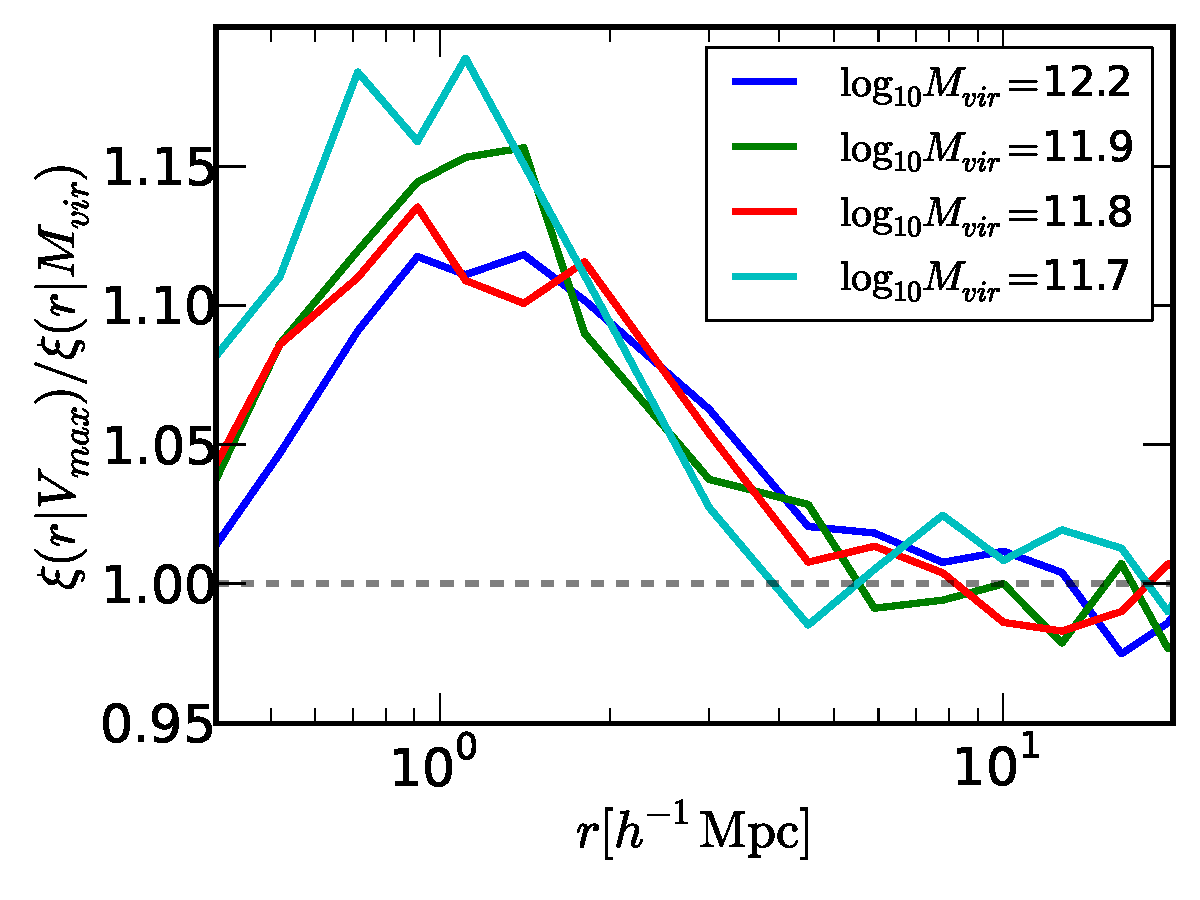
\includegraphics[width=0.5\columnwidth]{/Users/old_ts485/Desktop/biasVmax/plots/Bolshoi_andrew_smallScale}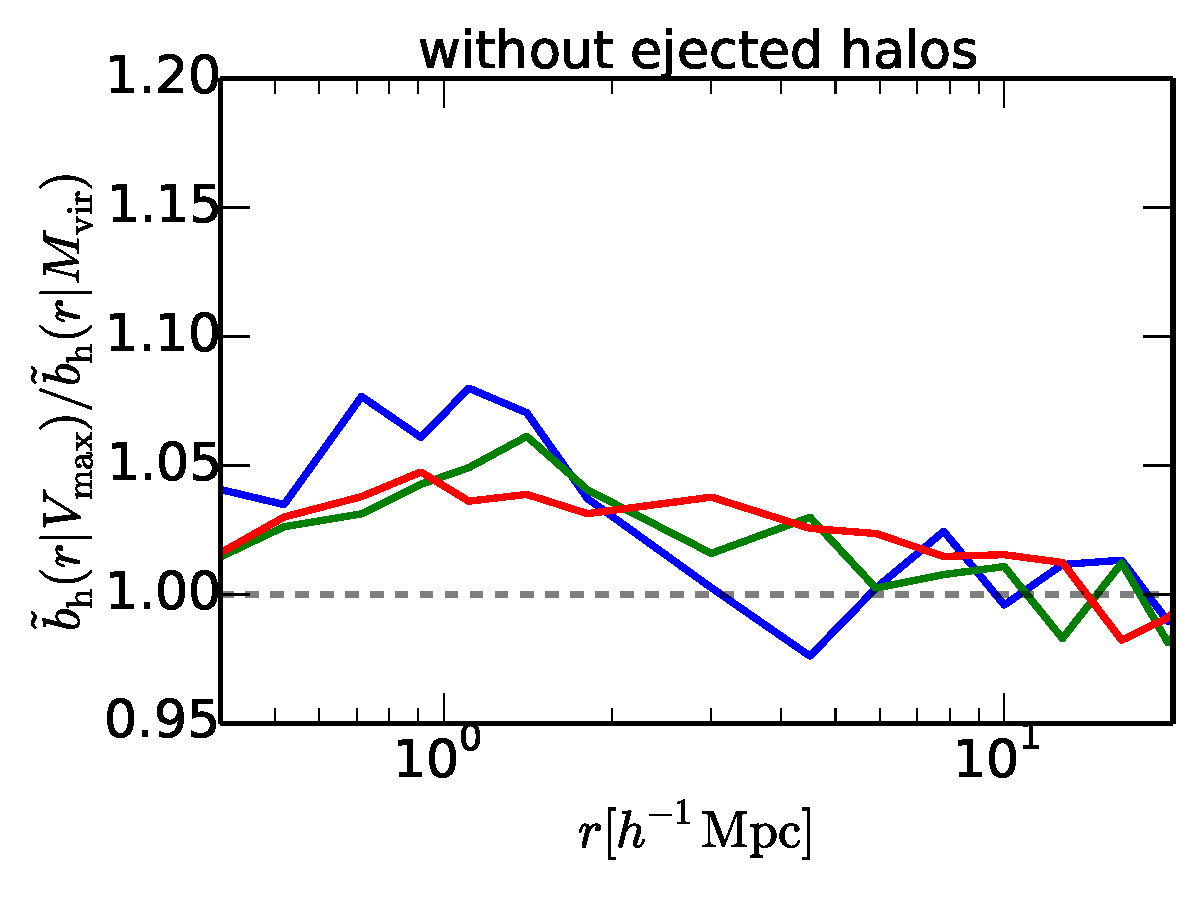
\includegraphics[width=0.5\columnwidth]{/Users/old_ts485/Desktop/biasVmax/plots/Bolshoi_andrew_smallScale_nonEj}

\caption{\label{fig:abundance_small}Ratio of halo-matter cross correlation
functions between$M_{{\rm vir}}$-based and $V_{{\rm max}}$-based
abundance matching samples with ejected halos (left) and without ejected
halos (right). The ratios are normalized by their linear biases. Each
line corresponds to different halo mass bins labeled in the plots.
With ejected halos, the halo biases computed from the $V_{{\rm max}}$-samples
have very different scale-dependence than the ones from the $M_{{\rm vir}}$-samples.
By removing those ejected halos, the difference is more or less removed.}
\end{figure}



\subsection{$\Delta\Sigma(r)$}

--Select a bin of Milky Way mass host halos, and select their number-density-matched
Vmax-selected equivalent. Use Peter Behroozi's stellar-to-halo mass
relation to estimate the stellar mass of the central galaxy that would
be found in these halos, then plot the halo-matter cross-correlation
as a function of scale, over-plotting the two results.

--want to show: We show that the galaxy-galaxy lensing signal of low-mass
centrals is impacted at the xxx-yyy\% level, in a highly scale-dependent
fashion, by the theoretical choice to empirically connect stellar
mass to either host halo Vmax or Mvir.


\section{Discussion}
\end{document}
